\documentclass[aspectratio=169,12pt]{beamer}
\usetheme{Madrid}
\usecolortheme{dolphin}
\usefonttheme{professionalfonts}
\setbeamertemplate{navigation symbols}{}
\setbeamertemplate{footline}{}

\usepackage[T1]{fontenc}
\usepackage[utf8]{inputenc}
\usepackage{graphicx}
\usepackage{amsmath,amssymb}
\usepackage{hyperref}
\usepackage{siunitx}
\usepackage{physics}
\usepackage{braket}
\graphicspath{{../2-qubit/figures/}{../3-portes_logiques/figures/}{../4-qiskit_base/figures/}{../5-mesure/figures/}{../6-plusieurs_qubits/figures/}}

\title[Rappel Jour 1]{Rappel Jour 1 : chapitres 2 à 6a}
\author{JAMOTTE Maxime, SCHOONEN Cédric}
\institute{Digital Learning Hub}
\date{}

\begin{document}

\begin{frame}
  \titlepage
\end{frame}

\begin{frame}{Chapitre 2 --- Vecteurs, qubit et superposition}
  \begin{columns}[T,onlytextwidth]
    \column{0.6\textwidth}
    \begin{itemize}
        \item Qubit = système à deux niveaux $\ket 0$ et $\ket 1$ (superposition possible).\\~\\
        \item Superposition \(\alpha\ket 0 + \beta\ket 1\) normalisée \(\rightarrow\)
         probabilités via \(|\alpha|^2,|\beta|^2\).\\~\\
        \item Etat d'un qubit représentable par  un vecteur.\\~\\
        \item Produit scalaire comme comparaison entre états (lien avec l'angle).        
    \end{itemize}
    \column{0.35\textwidth}
    \centering
    \includegraphics[width=\linewidth]{ket_base.png}
  \end{columns}
\end{frame}

\begin{frame}{Chapitre 3 --- Matrices et portes logiques}
    \begin{itemize}
      \item Opérations sur qubit par portes logiques quantiques = action matrice sur vecteur.\\~\\
      \item Portes quantiques 1 qubit: $H$ crée une superposition équilibrée, $X$ échange les amplitudes.\\~\\
      \item Composition de portes = produit de matrices agissant sur les vecteurs d'état.\\~\\
      \item Ordre des portes important.
    \end{itemize}
\end{frame}

\begin{frame}{Chapitre 4 --- Prise en main de Qiskit}
  \begin{columns}[T,onlytextwidth]
    \column{0.6\textwidth}
    \begin{itemize}
      \item États \(\ket 0\), \(\ket 1\) et portes ($H$, $X$) via \texttt{Statevector}, \texttt{Operator} et
       \texttt{evolve}.\\~\\
      \item Circuits équivalents avec \texttt{QuantumCircuit} puis \texttt{Statevector.from\_instruction}.\\~\\
      \item Visualiser rapidement un circuit: \texttt{qc.draw('mpl')}.\\~\\
      \item Exercices: ordres de portes différents \(\rightarrow\) résultats différents (non-commutativité).
    \end{itemize}
    \column{0.35\textwidth}
    \centering
    \includegraphics[width=0.9\linewidth]{gate_h_then_x.png}
  \end{columns}
\end{frame}

\begin{frame}{Chapitre 5 --- Mesure et valeurs propres}
  \begin{columns}[T,onlytextwidth]
    \column{0.6\textwidth}
    \begin{itemize}
      \item On mesure une observable, le résulat possible de la mesure est une de ses valeurs propres.\\~\\
      \item Probabilité d'obtenir une valeur propre via projection de l'état du système sur le vecteur propre associé, \(P = |\braket{\phi|\psi}|^2\).\\~\\
      \item Qiskit: ajouter un bit classique, \texttt{qc.measure}, probabilités = module carré des amplitudes.\\~\\
    \end{itemize}
    \column{0.35\textwidth}
    \centering
    \includegraphics[width=\linewidth]{measure_circuit.png}
  \end{columns}
\end{frame}

\begin{frame}{Chapitre 6 --- Systèmes à deux qubits et intrication}
  \begin{columns}[T,onlytextwidth]
    \column{0.6\textwidth}
    \begin{itemize}
      \item États à deux qubits: base \(\ket{00},\ket{01},\ket{10},\ket{11}\).\\~\\
      \item Produit tensoriel: $\ket{00} = \ket 0_2^{} \otimes \ket 0_1^{}$.\\~\\
      \item Intrication vs état produit et décomposition de Schmidt.\\~\\
      \item Génération d'une paire de Bell\\~\\
      \item Porte $C_X^{}$: applique $X$ sur un qubit si l'autre est dans l'état $\ket{1}$.\\~\\
      \item Porte $C_Z^{}$: applique $Z$ sur un qubit si l'autre est dans l'état $\ket{1}$.
    \end{itemize}
    \column{0.35\textwidth}
    \centering
    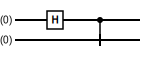
\includegraphics[width=0.8\linewidth]{bell_pair.png}
  \end{columns}
\end{frame}

\begin{frame}{Chapitre 6a --- Installation et workflow Qiskit}
\begin{itemize}
    \item Préparer l'environnement: venv, installation de \texttt{jupyter}, \texttt{qiskit}, \texttt{qiskit-ibm-runtime}, \texttt{qiskit-aer}.\\~\\
    \item Construire un circuit simple puis choisir la plateforme: QPU réel, faux QPU bruité ou simulateur AER.\\~\\
    %\item Transpilation/compilation du circuit vers la cible (\texttt{qiskit.compiler} ou \texttt{qiskit.transpiler}).
    \item Exécution et analyse: récupération des jobs; AER donne les distributions idéales, les QPU réels avec bruit.
    \end{itemize}
\end{frame}



\end{document}
